%%%%%%%%%%%%%%%%%  Debut du fichier Latex  %%%%%%%%%%%%%%%%%%%%%%%%%%%%%%
\documentclass[12pt,onecolumn]{article}
%\usepackage[style=numeric,maxnames=1,uniquelist=false]{biblatex}
\usepackage[backend=bibtex,style=numeric,minnames=4,maxnames=4,firstinits=true,sorting=none]{biblatex}  %backend=biber is 'better'  
\makeatletter
\def\blx@maxline{77}
\makeatother
\renewbibmacro{in:}{} % to not have the "In:" to indicate the review
\AtEveryBibitem{\clearfield{title}} % to remove the titles in the biblio
% no page info
\AtEveryBibitem{%
  \ifentrytype{article}{%
    \clearfield{pages}%
  }{%
  }%
}
% no language info
\AtEveryBibitem{\clearlist{language}}
% no language no page
\AtEveryBibitem{%
  \clearfield{volume}%
  \clearfield{number}}
% To avoid parenthesis if no year entry in bib file
\renewbibmacro*{issue+date}{%
  \ifboolexpr{not test {\iffieldundef{year}} or not test {\iffieldundef{issue}}}
    {\printtext[parens]{%
       \iffieldundef{issue}
         {\usebibmacro{date}}
         {\printfield{issue}%
          \setunit*{\addspace}%
          \usebibmacro{date}}}}
    {}%
  \newunit}


\ExecuteBibliographyOptions{isbn=false,url=false,doi=false,eprint=false}

%\bibliography{/Users/Ileyk/Documents/Bibtex/Hubble_fellowship_no_url} 
\addbibresource{/Users/Ileyk/Documents/Bibtex/CNRS_19.bib}
%%% Pour un texte en francais


%%\usepackage[applemac]{inputenc}
%\usepackage[francais]{babel}
	         % encodage des lettres accentuees
\usepackage[T1]{fontenc}
\usepackage[utf8]{inputenc}          % encodage des lettres accentuees
%\usepackage{graphicx}
%%\usepackage{graphicx} \def\BIB{}
\usepackage[paper=a4paper,left=1in,right=1in,top=1.5in,bottom=1.5in]{geometry}
\usepackage{multicol}
\usepackage{graphicx,wrapfig,lipsum} 
%\def\BIB{}
\usepackage{caption}
\usepackage{subcaption}
\usepackage[pdftex]{hyperref}
%\usepackage{natbib}
\usepackage{url}
\usepackage{perpage} %the perpage package
\MakePerPage{footnote} %the perpage package command
\hypersetup{
    colorlinks,%
    citecolor=black,%
    filecolor=black,%
    linkcolor=black,%
    urlcolor=blue     % can put red here to visualize the links
}

\usepackage{enumitem}
\usepackage{amssymb}

%\renewcommand{\refname}{}

\usepackage{floatrow}

\usepackage{fancyhdr}
\usepackage{lastpage}

\pagestyle{fancy}
\fancyhf{}
\rhead{Research summary}
\lhead{El Mellah Ileyk}
\rfoot{\thepage / \pageref{LastPage}}

\DeclareUnicodeCharacter{00A0}{ }

\usepackage{xspace}

%%% Quelques raccourcis pour la mise en page
\newcommand{\remarque}[1]{{\small \it #1}}
\newcommand{\rubrique}{\bigskip \noindent $\bullet$ }
\newcommand{\sgx}{SgXB\xspace}
\newcommand{\sgxs}{SgXBs\xspace}
\newcommand{\ulx}{ULX\xspace}
\newcommand{\sfxt}{SFXT}
\newcommand{\sg}{Sg\xspace}
\newcommand{\co}{CO\xspace}
\newcommand{\gw}{GW\xspace}
\newcommand{\gws}{GWs\xspace}
\newcommand{\grb}{GRB\xspace}
\newcommand{\grbs}{GRBs\xspace}
\newcommand{\eos}{EOS\xspace}
\newcommand{\mhd}{MHD\xspace}
\newcommand*{\hmxb}{HMXB\@\xspace}
\newcommand*{\hmxbs}{HMXBs\@\xspace}
\newcommand*{\lmxb}{LMXB\@\xspace}
\newcommand*{\rlof}{RLOF\@\xspace}
\newcommand*{\ns}{NS\@\xspace}
\newcommand*{\nss}{NSs\@\xspace}
\newcommand*{\bh}{BH\@\xspace}
\newcommand*{\bhs}{BHs\@\xspace}
\newcommand*{\eg}{e.g.\@\xspace}
\newcommand*{\ie}{i.e.\@\xspace}
\newcommand*{\aka}{a.k.a. \@\xspace}
\newcommand*\diff{\mathop{}\!\mathrm{d}}
\newcommand{\mystar}{{\fontfamily{lmr}\selectfont$\star$}}
\newcommand*{\msun}{$M_{\odot}$\@\xspace}
\newcommand*{\mdotstar}{$\dot{M}_{\text{\mystar}}$\@\xspace}
\newcommand*{\mdotacc}{$\dot{M}_{\text{acc}}$\@\xspace}
\newcommand*{\ledd}{$L_{\text{Edd}}$\@\xspace}


\newcommand{\ignore}[1]{}

%\renewcommand*\rmdefault{iwona}

%\pagenumbering{gobble}

%\bibliographystyle{abbrvnat}
%\setcitestyle{authoryear,open={((},close={))}}

%\renewcommand{\thefootnote}{\roman{footnote}}

% -------------------------------------------------
\newcommand{\horrule}[1]{\rule{\linewidth}{#1}} % Create horizontal rule command with 1 argument of height

\title{	
\vspace*{-2.5cm}
%\normalfont \tiny 
%%\textsc{Paris Diderot} \\ [25pt] % Your university, school and/or department name(s)
%\horrule{0.5pt} \\[0.4cm] % Thin top horizontal rule
\Large Speeding up the spinning top\\
\large How accretion sets the pace in High Mass X-ray Binaries  \\ % The assignment title
%\horrule{2pt} \\[0.5cm] % Thick bottom horizontal rule
}
\author{\tiny} % Your name
\date{\tiny }%\normalsize\today} % Today's date or a custom date
% -------------------------------------------------

%\makeatletter
%\def\@xfootnote[#1]{%
%  \protected@xdef\@thefnmark{#1}%
%  \@footnotemark\@footnotetext}
%\makeatother

%\usepackage[square,numbers,sort]{natbib}
%\usepackage{har2nat} % "natbib" is loaded automatically

%
%\let\oldthebibliography\thebibliography
%\renewcommand{\thebibliography}[1]{%
%  \oldthebibliography{#1}
%  \let\oldbibitem\bibitem
%  \let\oldtextsc\textsc
%  \def\oldbbland{et}
%  \newcounter{authorcount}
%  \def\bibitem[##1]##2{%
%    \let\textsc\oldtextsc
%    \let\bbland\oldbbland
%    \oldbibitem[##1]{##2}%
%    \let\textsc\mytextsc%
%    \let\bbland\mybbland
%    \setcounter{authorcount}{0}
%  }
%  \def\mybbland{\setcounter{authorcount}{0}\oldbbland}
%  \def\dropetal##1.{ \bbletal}
%  \def\mytextsc##1{%
%    \oldtextsc{##1}%
%    \stepcounter{authorcount}%
%    \ifnum\value{authorcount}=2\relax%
%      \expandafter\dropetal%
%    \fi%
%  }%
%}


\begin{document}

%\bibpunct{[}{]}{;}{n}{,}{,}

%%%%%%%%%%%%%%%%%%%%%%%%%  PREMIERE PAGE %%%%%%%%%%%%%%%%%%%%%%%%%%%%%%
%%% DANS CETTE PAGE, ON REMPLACE LES INDICATIONS ENTRE CROCHETS [...]
%%% PAR LES INFORMATIONS DEMANDEES
%%%%%%%%%%%%%%%%%%%%%%%%%%%%%%%%%%%%%%%%%%%%%%%%%%%%%%%%%%%%%%%%%%%%%%%

\renewcommand{\headrulewidth}{1pt}
\pagestyle{fancy}
\fancyhf{}
\rhead{Research proposal}
\lhead{El Mellah Ileyk}
\rfoot{\thepage / \pageref{LastPage}}

\vspace*{-1.2cm}
\begin{center}
\Large \textbf{The physics of kilonovae :}\\
\large What light curves tell us about the ultimate moments of merging neutron stars  
\end{center}
\normalfont

Massive stars live a forceful life during which they shape galaxies with their mechanical, radiative and chemical feedback. Most of them evolve in binary systems where the two stars orbit close enough to strongly interact \cite{Sana2012}. Last year, a gravitational wave detection granted us access to the very last moment this epic journey can lead to: the coalescence between two neutron stars (\ns, \cite{TheLIGOScientificCollaboration2017}). An intermediate step between these two stages are High Mass X-ray Binaries (\hmxbs), systems where stellar material is transferred from an evolved massive star to an orbiting compact remnant. The conditions of this transfer determine whether a double \ns with an orbital separation small enough to spiral-in and merge within a Hubble time will eventually be formed. 

Loss and exchange of angular momentum during this phase is a key problem to address. \ns are surrounded by an extended magnetosphere which plays a major role in the accretion process: the spin of the \ns in \hmxbs perturbs the accretion through magneto-centrifugal gating effects (\eg the propeller effect) and episodic mass outflows \cite{Bozzo2008}. Furthermore, the orbital separation has a direct impact on the mass transfer mechanism (Roche lobe overflow or wind accretion), on the geometry of the accretion flow and on the subsequent spiral-in time. Models are being developed to describe the formation of double \ns systems \cite{Tauris2017} but thorough and repeated observations of individual \hmxbs remind us how uncertain the proxies we rely on to compute evolutionary tracks can be. The two limit geometries of the accretion flow we currently rely on, either a thin disc or a spherical medium, do not cover the realistic intermediate case, with a stellar wind significantly beamed towards the accretor much before stellar evolution leads to stellar Roche lobe overflow. Within the current uncertainties on the properties of the winds of evolved massive star (mass loss rate, velocity profile, micro-structure), the geometry of the accretion flow when it reaches the magnetosphere fluctuates \cite{ElMellah2018}. Since the instantaneous torques at stake depend on whether the material forms a thin disc (prograde or retrograde) or remains essentially spherical as it is accreted, it has dramatic consequences on the spinning up or down of the accretor \cite{Ghosh1978,Shakura2012}. The transition from a regime to another induced by the inhomogeneities in the wind and the duty cycle determine the long term impact on the \ns spin.

A good illustration of our incomplete knowledge is given by the distribution and evolution of the \ns spin in Supergiant X-ray binaries (\sgxs, a sub-class of \hmxbs, see Figure\,\ref{fig:spin}). While some sub-classes of \hmxbs show common angular momentum trends, wind accreting \ns in \sgxs still defy theoretical expectations. They can display distinct long term phases of spinning up or down, which prove that the torque does not obey a random walk, and torque reversals are not necessarily associated with spectral or flux variations \cite{Hemphill2013}. 

The aim of this project is to gather these torque mechanisms into a consistent frame to evaluate the loss and transfer of angular momentum in the complex environment of \ns-hosting \sgxs following these core questions:

- - -

The discovery of the first gravitational wave (\gw) signal three years ago marked the dawn of a new astronomy \cite{Abbott2016}. Four decades after the indirect detection by Hulse \& Taylor in an inspiralling pulsar binary \cite{Hulse1974}, we are now fully able to capture the very last moments of the epic life of massive stars through the burst of \gw emitted when the compact remnants eventually merge. If the first detections were interpreted as merging black holes (\bhs), without any electromagnetic counterpart, a \gw signal from two merging neutron stars (\nss) was observed last year in association with a short gamma ray burst (\grb) and a subsequent luminous blue kilonova \cite{TheLIGOScientificCollaboration2017}. The crossed analysis of these three signals can unearth unvaluable information on a plethora of aspects : the equation-of-state (\eos) of condensed matter in \nss, the nucleosynthesis of the heaviest elements and new constrains on gravity in the strong field regime are only a few examples of the promising breakthroughs ahead.

Short \grbs are intense non-repeating flares of $10^{51}$ ergs released as gamma-rays over less than 2 seconds \cite{Berger2014}. With the discovery of an X-ray afterglow by \cite{Gehrels2005} came the identification of the host galaxy of a short \grb and the confirmation of their cosmological origin. They have long been thought to be powered by the accretion of a massive remnant disc onto the compact object formed after a \ns-\ns/\bh-\ns merger \cite{Eichler1989}. The interplay between accretion and rapid rotation of the central engine can drive a collimated ultra-relativistic outflow \cite{Piran2005}. Within this jet with typical opening-angles of a few degrees, relativistically beamed gamma-ray emission arises from energy dissipation via internal shocks \cite{Rees1992}. External shocks with circumburst material generate the aforementioned afterglow \cite{Kumar2015}.

Kilonovae are week-long supernovae-like transients, with a spectral peak ranging from near infrared to optical and a peak luminosity at 10$^{40-41}$erg$\cdot$s$^{-1}$ reached after a few days \cite{Tanaka2016,Metzger2017}. \cite{Tanvir2013} and \cite{Berger2013} associated kilonovae and \grbs by finding evidence for a significative near infrared excess in the late-time afterglow of a \grb. Kilonovae are thought to be produced by neutron-rich material ejected during a \ns-\ns/\bh-\ns merger : as the mildly relativistic cocoon expands, it is heated by radioactive decay \cite{Li1998}, a millisecond magnetar \cite{Yu2013} and/or fall-back accretion onto the central body \cite{Rosswog2007}. The relative contribution of these three mechanisms lies at the core of this research proposal whose main scientific questions are :

\begin{enumerate}
\item How neutron-rich are the different components of the ejecta?
\item How can the rotational energy of a fastly rotating magnetar remnant be transferred to the ejecta?
\item How could material falling back at later times heat the ejecta?
\end{enumerate}

A simplified sketch of the different components is displayed in Figure\,\ref{fig:sketch}.

\begin{figure}[!h]
\vspace*{0.3cm}
\floatbox[{\capbeside\thisfloatsetup{capbesideposition={right,center},capbesidewidth=9cm}}]{figure}[\FBwidth]
{\caption{Simplified sketch of the different physical components which can appear following a \ns-\ns/\bh-\ns merger. The central black dot stands for the merger remnant, either a \bh or a \ns (with possibly a finite lifetime). In the \ns scenario, a magnetosphere is expected (green dipole), along with a magnetar wind nebula containing copious amounts of neutrinos ($\nu$). Material ejected in the equatorial plane of the fastly rotating remnant (spin $\omega$) might sometimes form a disc from which can depart a neutrino-driven wind. The two jets responsible for the short \grb are represented in black (with double lines indicating internal and external shocks). The kilonova (in red) comes from outflowing material. The details of these pictures depend strongly on the initial merger and the nature of the remnant.}\label{fig:sketch}}
{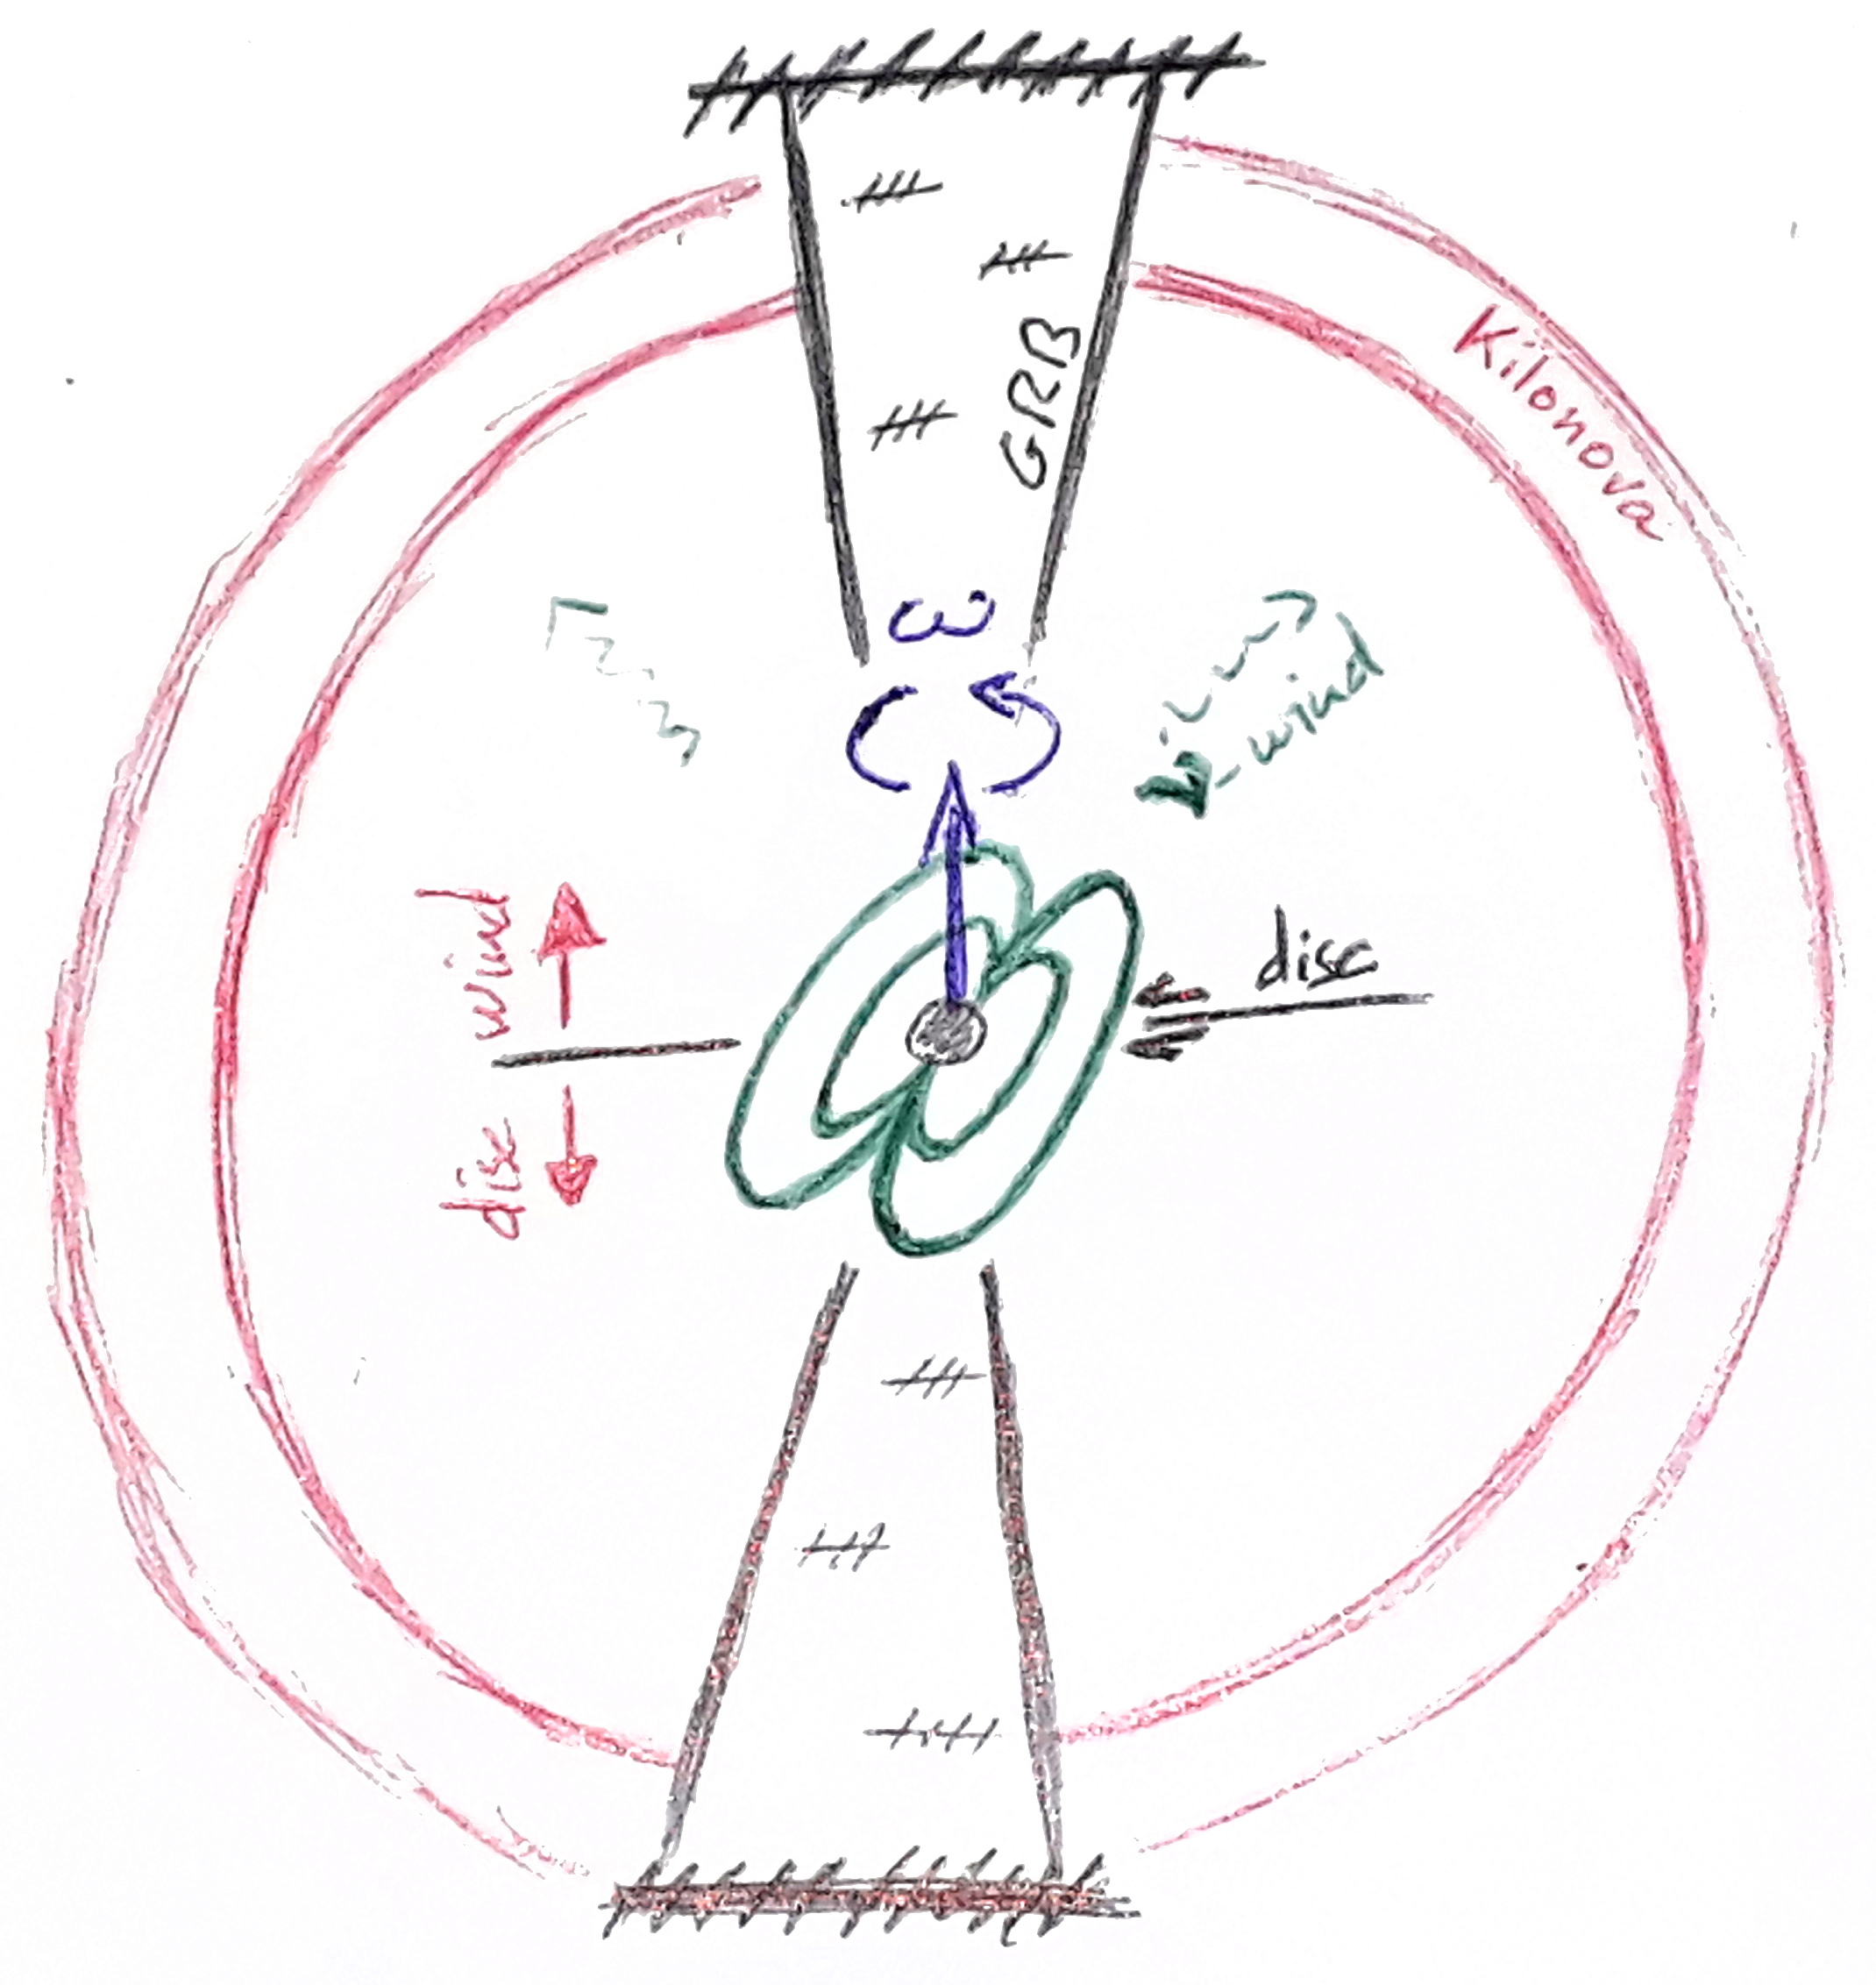
\includegraphics[width=7cm]{Figures/sketch_GRB_kilonova.jpg}}
\vspace*{-0.4cm}
\end{figure}

\section{A site for nucleosynthesis of neutron-rich elements}

Kilonovae have long been suspected to be the main site for the nucleosynthesis of the heaviest elements \cite{Lattimer1974}, along with core-collapse supernovae \cite{MacFadyen1999}. Due to their dense neutron-rich content (\ie low electron fraction), kilonovae can be the stage of rapid neutron-capture by seed nuclei like Iron, the so-called "r-process". The yield of this nucleosynthesis and the associated heating of the kilonova can be derived from nuclear reaction networks \cite{Metzger2010} and the electron fraction, with higher yields for lower electron fractions. However, the electron fraction can only be deduced once we properly account for neutrino-irradiation : neutrino absorption reactions on nucleons increase the electron fraction of the material and might inhibit the formation of heavy elements such as lanthanides. Since the opacity of lanthanides can quickly dominate and determine the properties of a kilonova light curve, we need to figure out how neutrinos interact with the different components during a \ns-\ns/\bh-\ns merger.

At the LUTh, Micaela Oertel's team developed a computationally affordable method to solve neutrino transport in the context of core-collapse supernovae \cite{Peres2011}. I would like to extend this treatment to \ns-\ns/\bh-\ns mergers and implement it in a form suitable to be used in conjunction with the finite volume code \texttt{MPI-AMRVAC} (Message Passing Interface - Adaptive Mesh Refinement Versatile Advection Code) I have been using and co-developing for the last five years (see section XXX). During my postdoctoral years, I have worked on different schemes to solve the radiative transfer equations : methods inspired from long characteristics with Jon Sundqvist (KU Leuven), flux-limited diffusion and an alternating directional implicit scheme with Nicolas Moens (a PhD student I co-supervise with Jon Sundqvist) and multi-grid solvers with Jannis Teunissen (CWI Amsterdam). Although physical differences exist between neutrinos and photons, these numerical techniques share many common points with the ones developed for neutrino transport. Coupling the micro-Physics to the flow dynamics has become an absolute requirement to improve our understanding of these high temperature environments. Another human asset to connect the heating of the merger surroundings to the observed light curves is the presence of Frédéric Vincent at the LUTh for the last couple of years. The general relativity code he led the development of, \texttt{GYOTO} \cite{Vincent2011}, could prove useful to appreciate transport mechanisms in the immediate vicinity of the compact object.

\section{Spinning down of a magnetar remnant}

Extraction of the huge rotational energy contained in a millisecond magnetar (\ie with a magnetic field strength above 10$^{14}$G) via electromagnetic torques might significantly enhance the electromagnetic emission from \ns-\ns mergers. It could be a major source of heating for the kilonova, provided it can sustain a high spinning down luminosity for long enough (see Figure\,\ref{fig:spinning_down}). The modalities of the coupling between the plasma and the magnetosphere depend strongly on the relative extension of the magnetosphere with respect to the corotation radius, the radius at which the period of a Keplerian orbit matches the \ns spin period \cite[see \eg the propeller effect described in][]{Bozzo2008}. This collisionless plasma has been widely studied by Fabrice Mottez (LUTh) whose expertise would be extremely valuable to address these questions. 

With Zakaria Meliani (LUTh), we are currently working on magneto-hydrodynamics (\mhd) setups to compute torques applied to \nss in X-ray binaries. Thanks to the radially stretched meshes I implemented during my PhD, we could adapt these setups to kilonovae and characterize the impact of the interaction with the spinning down magnetosphere on the dynamics of the flow. 

This work would bring decisive keys to shed unprecedented light on another topic of interest of the LUTh : the internal structure of \nss and their \eos. When a \ns-\ns merger occurs, three different types of remnants can be formed, from the lighter to the heavier : a stable \ns, a supramassive \ns sustained by its solid body rotation, or a body quickly collapsing into a \bh (for simplicity, I include hypermassive \ns in this last case). While a stable magnetar can participate indefinitely in the heating of the kilonova (although at lower levels as time goes by), a supramassive \ns will collapse into a \bh once it spins down below a certain threshold : in this case, only a fraction of the rotational energy can be extracted before the \ns collapses. The possibility of a short or long-lived \ns remnant could not be ruled out in the \gw signal of the double neutron star merger of last year.

In Figure\,\ref{fig:spinning_down}

\begin{figure}[!h]
\vspace*{0.3cm}
\floatbox[{\capbeside\thisfloatsetup{capbesideposition={right,center},capbesidewidth=6cm}}]{figure}[\FBwidth]
{\caption{Rates of \ns rotational energy decay as a function of time. Different \ns magnetic field strengths and masses are considered, and standard parameters taken from \cite{Metzger2017} are used. While a 2M$_{\odot}$ \ns does not need centrifugal support to avoid collapsing into a \bh, a 2.4M$_{\odot}$ \ns might qualify as a supramassive \ns and collapse once it has evacuated too much rotational energy (green dots). See text for more details.}\label{fig:spinning_down}}
{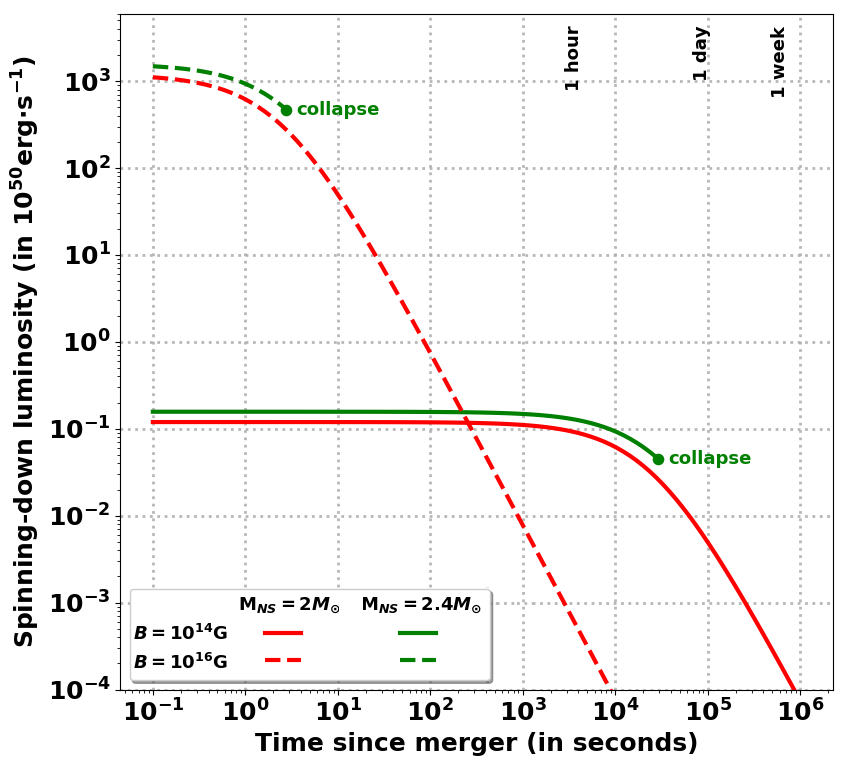
\includegraphics[width=10cm]{Figures/spinning-down_luminosity.png}}
\vspace*{-0.4cm}
\end{figure}

\phantom{\cite{ElMellah2016a,ElMellah2018a,Xia2017,Rappaport:2012wi,Rappaport2013,SanchisOjeda:2014ww}}
%%\subsubsection*{References}
\vspace*{-1.2cm}
\setlength\bibitemsep{0pt}
%%\scriptsize
%\bibliographystyle{ieeetr}
%\bibliography{/Users/Ileyk/Documents/Bibtex/Hubble_fellowship_no_url}

%\bibliographystyle{ieeetr}
\printbibliography


\end{document}
%%%%%%%%%%%%%%%%%  Fin du fichier Latex  %%%%%%%%%%%%%%%%%%%%%%%%%%%%%%

